\chapter{Aprendizado de Máquina}
Como \citet{rezende2003sistemas} descreve, aprendizado de máquina é uma área de Inteligência Artificial no qual sistemas são capazes de adquirir conhecimento automaticamente. Um sistema de aprendizado é programa capaz de tomar decisões baseado em experiências acumuladas. Dessa forma, a partir de um conjunto de dados, chamados conjunto de treinamento, são inferidos um conjunto de parâmetros a serem utilizados em um modelo parametrizado.

\section{Definições}

Algumas breves definições serão apresentadas com a finalidade de ambientar o leitor nos temas discutidos neste capítulo.

\begin{description}
\item \textbf{Conjunto de exemplos}: É o conjunto de entidades modeladas no problema. Essas entidades poderiam ser pessoas, máquinas, imagens, sinais de som, enfim qualquer objeto que se queira estudar.

\item \textbf{Características}: É um conjunto ordenado de valores que descrevem um exemplo. A escolha das características utilizadas para representar os exemplos traz consequências diretas ao problema.

\item \textbf{Etiqueta}: É a classe que um exemplo particular pertence. Essa definição será utilizada para descrever os diversos tipos de cenário que os dados podem se encontrar, por exemplo nem sempre as etiquetas estão disponíveis.

\item \textbf{Função Custo}: É a função que mede quanto o modelo se enquadra ao conjunto de exemplos. Por exemplo, em uma regressão linear utiliza-se a soma das distâncias entre as características dos exemplos e o modelo linear que se quer utilizar para generalizar essas características.
\end{description}


\section{Categorias de Problemas}

Dentro do universo de problemas que são resolvidos pelas técnicas de aprendizado de máquina, é possível classificá-los em cinco categorias \citep{mohri2012foundations}.

\begin{description}
\item \textbf{Classificação}: Decidir a classe de um exemplo partindo das suas características, por exemplo decidir qual dígito foi escrito conhecendo uma imagem de dígito escrita a mão.
\item \textbf{Regressão}: Determinar um valor real para cada exemplo, por exemplo calcular o risco de um paciente ter contraído câncer a partir de imagens e resultados de exames.
\item \textbf{Ordenação}: Ordenar os exemplos a partir de algum critério, por exemplo listar produtos por relevância a partir das palavras chaves da busca do usuário.
\item \textbf{Agrupamento}: Particionar os exemplos em regiões homogêneas, por exemplo identificar comunidades dentro de redes sociais massivas.
\item \textbf{Redução de Dimensionalidade}: Representar o conjunto de exemplos com um número reduzido de dimensões, por exemplo comprimir imagens para processamento de imagens.
\end{description}

Neste projeto o objetivo é identificar grupos com padrão de comportamento semelhantes. A expectativa é que o comportamento dos bots formem grupos divergentes dos usuários legítimos. Todavia, nem toda máquina pertencente a esse grupo divergente está infectada, o que se quer garantir é um número de reduzido, da ordem das dezenas, de máquinas suspeitas para serem analisadas, dessa forma o usuário poderá dar atenção aos casos divergentes.

\section{Cenários dos Dados}

Categoriza-se \citep{mohri2012foundations} diversos cenários para os algoritmos de aprendizado, esses cenários são fortemente influenciados pelas condições dos dados de treinamento. Dentre os quais os três principais são:

\begin{description}
\item \textbf{Aprendizado Supervisionado}: O modelo tem acesso a dados com os resultados de saída já esperados, ou etiquetados, como lê-se na literatura. Os problemas mais comuns desse tipo de cenário são classificação, regressão e ordenação.

\item \textbf{Aprendizado Não Supervisionado}: Só se dispõe do conjunto de exemplos para treinamento sem etiquetas. Geralmente é mais utilizado para classificação, agrupamento e redução de dimensionalidade

\end{description}

E ainda há outros possíveis cenários ainda mais complexos e específicos, como o cenário semi-supervisionado, o qual os exemplos estão parcialmente etiquetados. Os demais cenários não foram catalogados neste trabalho por causa da exaustiva lista.

No caso deste trabalho, algumas máquinas identificadas pelo IP foram confirmadas como bots, mas não há garantia de que sejam os únicos bots na rede. O algoritmo se vê num cenário não supervisionado, mas os desenvolvedores validam os resultados a partir dos bots já conhecidos.

Note que se as máquinas conhecidamente suspeitas não se encontrarem no grupo divergente, o sistema falhou.

\section{Algoritmos de Agrupamento}

Existem diversas definições para grupos de entidades similares \citep{faceli2011inteligencia}, dentre elas podem ser citadas:
\begin{description}
\item \textbf{Grupos bem separados}: Cada exemplo de um grupo está mais próximo de outro exemplo do mesmo grupo do que a qualquer outro ponto não pertencente a ele. Essa definição se assemelha bastante à abordagem de aprendizado K vizinhos mais próximos num cenário supervisionado.
\item \textbf{Grupo baseado em centro}: Cada exemplo do grupo está mais próximo do centroide do próprio grupo do que do centroide de qualquer outro grupo. Essa é a premissa básica do K-médias.
\item \textbf{Grupo contínuo}: Qualquer exemplo de um grupo está mais próximo a um ou mais exemplos do mesmo grupo do que a qualquer outro exemplo não pertencente ao grupo. Essa definição é bastante similar ao Grupo bem separado. Porém, no Grupo contínuo basta estar mais próximo a um conjunto reduzido do mesmo grupo, diferente do bem separado que precisa estar mais próximo a todos do mesmo grupo.
\item \textbf{Grupo baseado em densidade}: Um grupo é uma região de alta densidade, separada de outras regiões de alta densidade por zonas de baixa densidade.
\item \textbf{Grupo baseado em similaridade}: Cada exemplo é comparado através de uma matriz de similaridade para então se tomar a decisão de agrupamento.
\end{description}

Cada definição induz uma abordagem de algoritmo diferente. Para esse trabalho, decidiu-se utilizar o modelo mais simples que é o de Grupo baseado em centro para resolver o problema. O algoritmo utilizado que é baseado na definição escolhida é o algoritmo de K-médias que será apresentado detalhadamente na seção \ref{sec:kmeans}. Porém, outros modelos, como o baseado em similaridade, podem vir a ser úteis, já que o objetivo desse trabalho é identificar grupos baseado em comportamentos tipicamente divergentes do comportamento comum.

\section{K-Médias}\label{sec:kmeans}

Segundo \citet{witten2011data}, K-Médias é um algoritmo de aprendizado iterativo baseado na distância geométrica. Inicialmente o algoritmo inicializa \textit{K} centroides em posições distintas. Cada exemplo, então, é associado ao centroide mais próximo. Em seguida o centroide atualiza sua posição para a média das posições dos pontos associados a ele. A partir de então recomeça o ciclo, são reassociados os pontos que estão mais próximos do centroide em sua nova posição.

Note que a função custo que se espera minimizar é a soma de todas as distâncias entre os exemplos e seus respectivos centroides, como descrito na seguinte equação

\[
\sum_{i=1}^{n} \lVert cent(\mathbf{X_{i}}) - \mathbf{X_{i}} \rVert
\]

O qual \(cent(\mathbf{X})\) é a função que retorna o centroide mais próximo das coordenadas \(\mathbf{X}\)

\begin{figure}
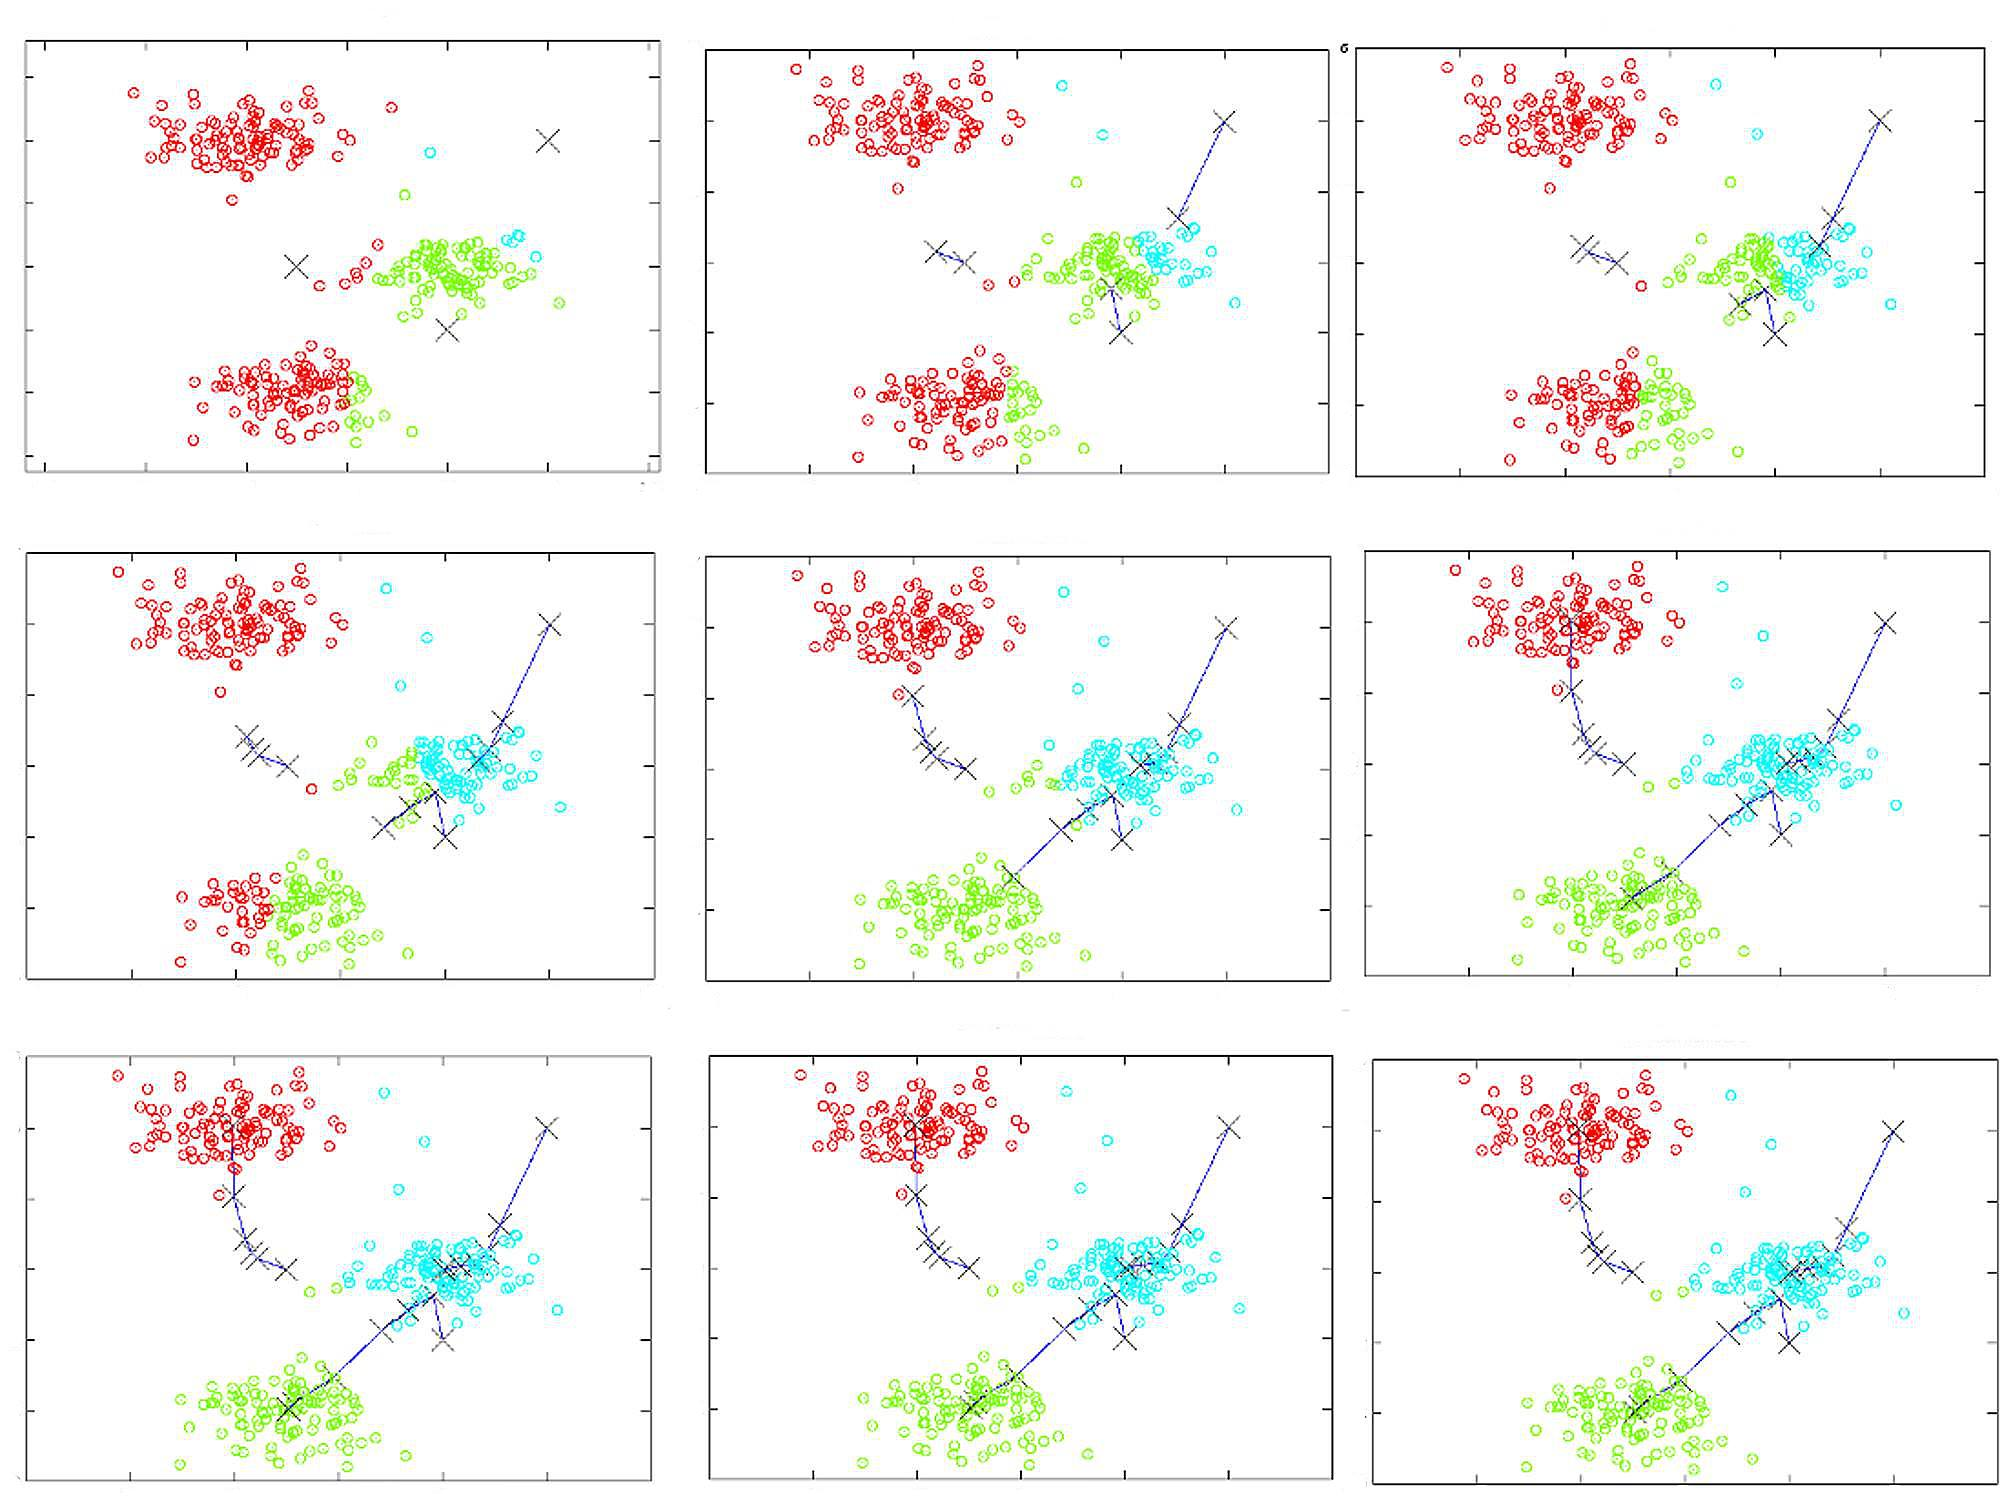
\includegraphics[width=\textwidth]{k_means_example}
\caption[Aplicação do K-Médias]{Aplicação do K-Médias} \label{fig:k_means_example}
\end{figure}

Pode-se visualizar a aplicação da técnica em dados bidimensionais com três grupos na figura \ref{fig:k_means_example}. Além disso, nota-se que a convergência é rápida, nesse caso em apenas 9 iterações chegou-se a um resultado satisfatório. Além disso, espera-se uma quantidade de máquinas da ordem de \(10^4\), como o algoritmo K-Médias é linear tanto na decisão do grupo para cada instância quanto no cálculo do novo centroide, a temporização do algoritmo é muito baixa.

\subsection{Determinação do Número de Grupos}

Para a operação plena do algoritmo é necessário que seja informada a quantidade de grupos que são buscados. A visualização é facilitada quando é possível avaliar visualmente os dados, como na figura \ref{fig:k_means_example}, mas não é possível realizar o mesmo procedimento quando os exemplos têm mais que três dimensões, como no caso deste projeto.

\begin{figure}
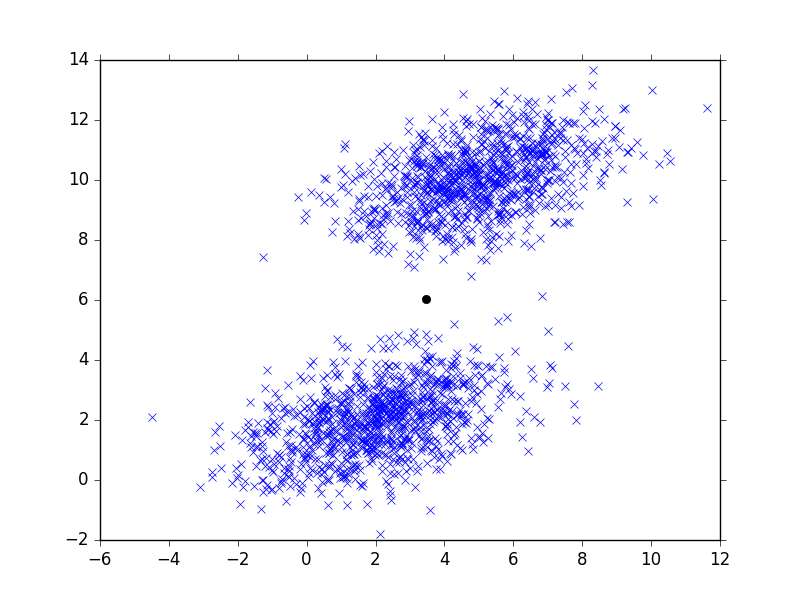
\includegraphics[width=\textwidth]{between_two_clusters}
\caption[Centroide Pouco Representativo]{Centroide Pouco Representativo} \label{fig:between_two_clusters}
\end{figure}

Além disso, se por um lado, pode-se carecer de centroides levando a cenários como na figura \ref{fig:between_two_clusters}, no qual o centroide não generaliza os dados, por outro, como é possível visualizar na figura \ref{fig:cluster_overfitting}, um grupo pode acabar se separando por centroides desnecessários.

\begin{figure}[htbp]
\centering
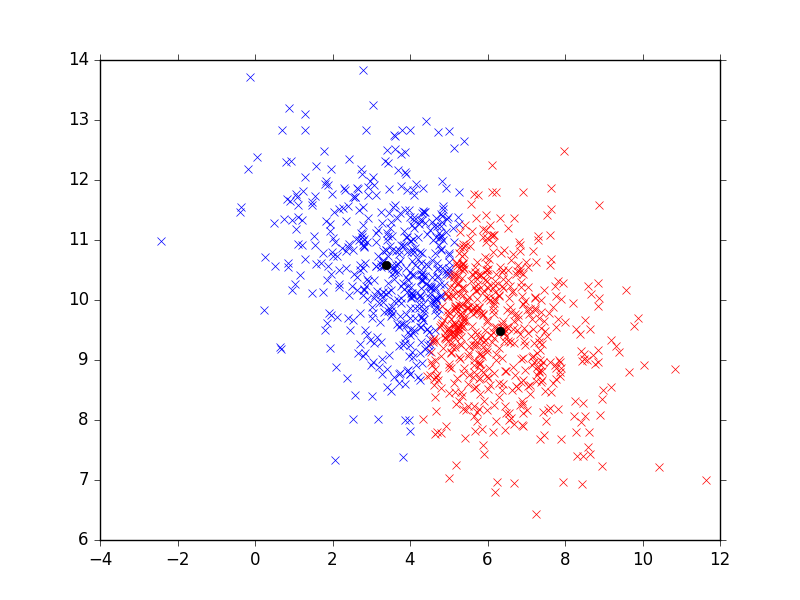
\includegraphics[scale=0.5]{cluster_overfitting}
\caption[Grupo Dividido]{Grupo Dividido} \label{fig:cluster_overfitting}
\end{figure}

Para resolver esse problema utiliza-se o Método \textit{Elbow} \citep{kodinariya2013review}. Trata-se de um método baseado na aferência visual no qual procura-se o ponto em que a adição de um novo centroide não implica mais na redução drástica da função custo criando um bico, ou cotovelo. Esse efeito é observado na figura \ref{fig:elbow}

\begin{figure}[htbp]
\centering
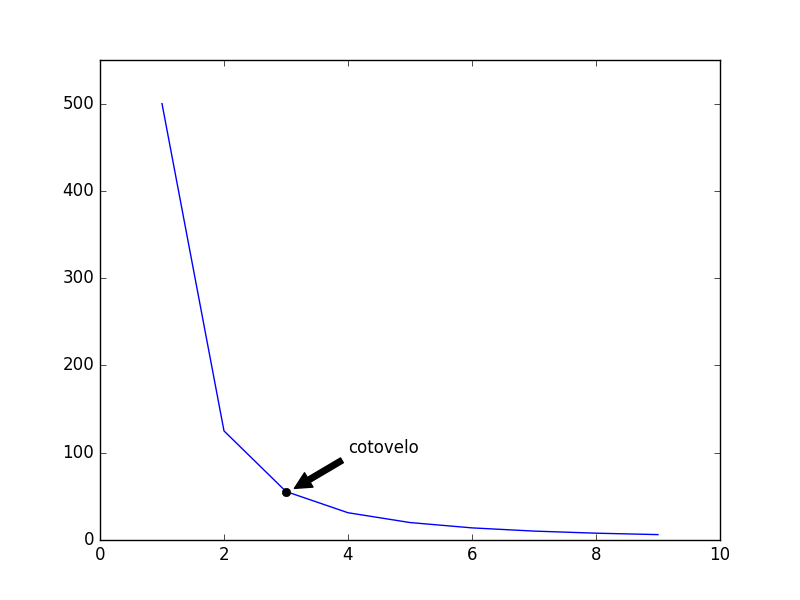
\includegraphics[scale=0.5]{elbow}
\caption[Ponto Crítico da Otimização]{Ponto Crítico da Otimização} \label{fig:elbow}
\end{figure}

O artigo \citet{kodinariya2013review} também cita outros métodos com critérios matemáticos menos subjetivos. Porém, decidiu-se utilizar o Método \textit{Elbow} para uma análise inicial, por fins de simplicidade. No capítulo \ref{ch:discussion} relativo aos experimentos, esse método será avaliado para os dados que foram utilizados neste trabalho.

\subsection{Inicialização do Centroides}

A inicialização dos centroides é um problema a ser considerado ao se aplicar o K-Médias, pois dependendo do estado inicial a função custo final pode acabar em um mínimo local por causa do estado inicial.

Para ilustrar, considere o cenário em que dois centroides acabam inicializados muito próximos e dentro de um grupo denso de pontos e bastante separado dos demais grupos. Neste cenário o modelo acabará dividindo o grupo em 2 separados deixando os demais centroides desamparados na tentativa de modelar os demais grupos.

Para solucionar os problemas da inicialização como o do exemplo citado, foi proposto o algoritmo K-means++ \citep{arthur2007k}, que modifica a função densidade de probabilidade a cada centroide instanciado, de forma que a densidade de probabilidade do centroide ser criado próximo a um ponto já instanciado seja baixa.
